%!TEX root=../../autopilot.tex
\section{Tasks}
\label{sec:tasks}
\begin{marginfigure}[0cm]
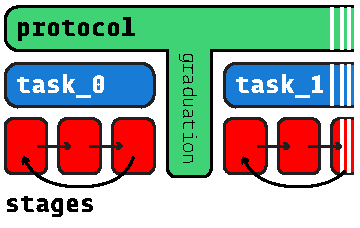
\includegraphics[]{figures/side_17_protocol.pdf}
\caption{Protocols consist of one or multiple tasks, tasks consist of one or multiple stages. Completion of all of a task's stages constitutes a trial, and meeting some graduation criterion like accuracy progresses a subject between tasks.}
\label{fig:taskstx}
\end{marginfigure}

Behavioral experiments in Autopilot are centered around \textbf{tasks}. Tasks are Python classes that describe the parameters, coordinate the hardware, and perform the logic of the experiment. Tasks may consist of one or multiple \textbf{stages} like a stimulus presentation or response event, completion of which constitutes a \textbf{trial} (Figure \ref{fig:taskstx}). Stages are analogous to states in the finite state machine formalism. 

Multiple tasks are combined to make \textbf{protocols}, in which animals move between tasks according to "graduation" criteria like accuracy or number of trials. Training an animal to perform a task typically requires some period of shaping where they are familiarized to the apparatus and the structure of the task. For example, to teach animals about the availability of water from "nosepoke" sensors, we typically begin with a "free water" task that simply gives them water for poking their nose in them. Having a structured protocol system prevents shaping from relying on intuition or ad hoc criteria.


\subsection{Task Components}
\label{sec:taskcomponents}

The following is a basic two-alternative choice (2AFC) task---a sound is played and an animal is rewarded for poking its nose in a designated target nosepoke. While simple, it is included here in full to show how one can program a task, including an explicit data and plotting structure, in roughly 60 lines of generously spaced Python.

\clearpage

Every task begins by describing four elements: 

1) the task's parameters, 2) the data that will be collected, 3) how to plot the data, and 4) the hardware that is needed to run the task.

\begin{pythoncode*}{label = \texttt{\textbf{task - parameters}}}
class Nafc(Task):
    class Params(Task_Params):|$\tikzmark{params}$|
        stim: Sounds = Field(...,          |$\tikzmark{tag}$|
            description = "Sound Stimuli") 
        reward: units.mL|$\tikzmark{units}$| = Field(...,
            description = "Reward Volume (mL)" |$\tikzmark{type}$|
        )

    class TrialData(Trial_Data): |$\tikzmark{data}$|
        target: Side = Field(..., 
            description="Side (L, R) of the correct response")
        correct: bool = Field(...,
            description="Response matched target")

    PLOT = {} |$\tikzmark{plot}$|
    PLOT['data']  =  {'target'  : 'point',
                      'correct' : 'rollmean'},
    # n trials to roll window over
    PLOT['params'] = {'roll_window' : 50}

    HARDWARE = { |$\tikzmark{hardware}$|
        'POKES':{
            'L': 'Digital_In',
            'R': 'Digital_In'
        },
        'PORTS':{
            'C': 'Solenoid', |$\tikzmark{hwdetail}$|
        }
    }
\end{pythoncode*}
%
\begin{tikzpicture}[overlay, remember picture]
\draw[<-] (pic cs:params) ++(0,0.1) to[left] ++(6.0,0) --++(0,0.75) --++(0.2,0)node[below right, yshift=8pt, text width=2.4in]{\normalfont \textcolor{red}{1) A \texttt{Task\_Params} model} defines what parameters are needed to run the task.};
\draw[decorate, decoration={brace,amplitude=5pt}] ($(pic cs:tag)+(0,11pt)$) -- ($(pic cs:tag)-(0,14pt)$) coordinate[midway](midWay);
\draw[-] (midWay)++(.15,0) --++(3.9,0) node[below right, yshift=8pt, text width=2.4in]{We use \texttt{Field} objects as before, and can also use some special types like \texttt{Sounds} to declare complex parameters};
\draw[<-] (pic cs:units) ++(-0.1,-0.2) --++(0,-0.5) --++(7.2,0)node[below right, yshift=8pt, text width=2.4in]{\normalfont \texttt{units} work like numbers but avoid ambiguity, so eg. the \texttt{Solenoid} class below knows this is a volume, rather than a duration};
\draw[<-] (pic cs:data) ++(0,0.1) to[left] ++(5.5,0) --++(0,-0.7) --++(0.2,0)node[below right, yshift=8pt, text width=2.4in]{\textcolor{red}{2) A \texttt{Trial\_Data} model} defines what data will be returned from the task. };
\draw[<-] (pic cs:plot) ++(0,0.1) to[left] ++(8.7,0)node[below right, yshift=8pt, text width=2.4in]{\textcolor{red}{3) A \texttt{PLOT} dictionary} maps the data output to graphical elements in the GUI. (In future versions this will be incorporated into the \texttt{Field}s of \texttt{TrialData})};
\draw[<-] (pic cs:hardware) ++(0,0.1) to[left] ++(8.2,0)node[below right, yshift=8pt, text width=2.4in]{\textcolor{red}{4) A \texttt{HARDWARE} dictionary} that describes what hardware will be needed to run the task.};
\draw[<-] (pic cs:hwdetail) ++(0,0.1) to[left] ++(6.3,0)node[below right, yshift=8pt, text width=2.4in]{The specific implementation of the hardware (eg. where it is connected, how to interact with it) is independent of the task. The task just knows about a \texttt{PORT} named \mintinline{python}{'C'} that is a \texttt{Solenoid}.};
\end{tikzpicture}

Created tasks receive some common methods, like input/trigger handling and networking, from an inherited metaclass. Python inheritance can also be used to make small alterations to existing tasks\sidenote{An example of subclassing a generic 'Task' class is included in Autopilot's \href{http://docs.auto-pi-lot.com/guide.task.html}{user guide}} rather than rewriting the whole thing. The GUI will use the \texttt{Params} model and the \texttt{PLOT} dictionary to generate forms for parameterizing the task within a protocol and display the data as it is collected. The \texttt{Subject} class will use the \texttt{TrialData} model to create HDF5 tables to store the data, and the \texttt{Task} metaclass will instantiate the described \texttt{HARDWARE} objects from their system-specific configuration in the \texttt{prefs.json} file so they are available in the rest of the class like \mintinline{python}{self.hardware['POKES']['L'].state}

\clearpage

\subsection{Stage Methods}

The logic of tasks is described in one or a series of methods (stages). The order of stages can be cyclical, as in this example, or can have arbitrary logic governing the transition between stages.
\vspace{10pt}

\begin{pythoncode*}{label = \texttt{\textbf{task - methods}}, firstnumber=last}
    def __init__(self, params:'Nafc.Params'): |$\tikzmark{init}$|
        self.stim_mgr = Stim_Manager(params.stim)
        self.reward   = Reward_Manager(params.reward) |$\tikzmark{mgrs}$|

        stage_list  = [self.discrim, self.reinforcement] |$\tikzmark{stages}$|
        self.stages = itertools.cycle(stage_list)

        self.init_hardware()
        next(self.stages)() |$\tikzmark{start}$|

    def discrim(self):
        target, wrong, stim = self.stim_mgr.next() |$\tikzmark{stim_mgr_2}$|
        self.target = target

        self.triggers[target] = [
            self.hardware['PORTS']['C'].open, |$\tikzmark{triggerset}$|
            lambda: next(self.stages)()]
        self.triggers[wrong] = lambda: next(self.stages)()

        self.node.send('DATA', {'target':target}) |$\tikzmark{data1}$|

        stim.play()

    def reinforcement(self, response): |$\tikzmark{args}$|
        if response == self.target: |$\tikzmark{data2}$|
            self.node.send('DATA', {'correct':True})
        else:
            self.node.send('DATA', {'correct':False})

        next(self.stages)() |$\tikzmark{callagain}$|
\end{pythoncode*}
\begin{tikzpicture}[overlay, remember picture]
\draw[<-] (pic cs:init) ++(0,0.1) to[left] ++(3.5,0) --++(0,1.5) --++(0.2,0)node[below right, yshift=8pt, text width=2.4in]{In Python, \mintinline{python}{def} defines new methods. The \mintinline{python}{__init__} method is called when a new object is initialized};
\draw[decorate, decoration={brace,amplitude=5pt}] ($(pic cs:mgrs)+(0,22pt)$) -- ($(pic cs:mgrs)-(0,3pt)$) coordinate[midway](midWay);
\draw[-] (midWay)++(.15,0) --++(2.05,0) --++(0,0.6) --++(0.2,0)node[below right, yshift=8pt, text width=2.4in]{\hyperref[sec:managers]{Managers} control stimulus and reward delivery, so users can, for example, continually synthesize new stimuli or implement adaptive rewards};
\draw[decorate, decoration={brace,amplitude=5pt}] ($(pic cs:stages)+(0,8pt)$) -- ($(pic cs:stages)-(0,18pt)$) coordinate[midway](midWay);
\draw[-] (midWay)++(.15,0) --++(1.5,0) --++(0.2,0)node[below right, yshift=8pt, text width=2.4in]{Stages are combined into an object that (in this case) continually cycles through them when its \mintinline{python}{next()} method is called.};
\draw[<-] (pic cs:start) ++(0,0.1) --++(6.35,0) --++(0,0) --++(0.2,0)node[below right, yshift=8pt, text width=2.4in]{This starts the task by retrieving the first stage and then calling it.};
\draw[<-] (pic cs:stim_mgr_2) ++(0,0.1) to[left] ++(2.85,0)node[below right, yshift=8pt, text width=2.4in]{The stimulus manager returns which port will be the target and the sound to be played.};
\draw[decorate, decoration={brace,amplitude=5pt}] ($(pic cs:triggerset)+(0,22pt)$) -- ($(pic cs:triggerset)-(0,20pt)$) coordinate[midway](midWay);
\draw[-] (midWay)++(.15,0) --++(3.3,0) --++(0,0.4) --++(0.2,0)node[below right, yshift=8pt, text width=2.4in]{A sequence of triggers is set: if the target port is poked, a reward will be delivered and the next stage will be called. A \mintinline{python}{lambda} function indicates not to call the method \textit{now}, but only when triggered.};
\draw[<-] (pic cs:data1) ++(0,0.1) to[left] ++(2.75,0) --++(0,-0.25) --++(0.2,0)node[below right, yshift=8pt, text width=2.4in]{The task has a networking object that asynchronously streams data back to the user-facing terminal};
\draw[<-] (pic cs:args) ++(0,0.1) to[left] ++(4.75,0)node[below right, yshift=8pt, text width=2.4in]{In this example, the response port is passed from the trigger handling function. If it matches the stored target variable, the animal answered correctly.};
\draw[<-] (pic cs:callagain) ++(0,0.1) to[left] ++(6.25,0) --++(0,0.5) --++(0.2,0)node[below right, yshift=8pt, text width=2.4in]{Finally, the task is repeated by calling the next stage.};
\end{tikzpicture}%
%
Autopilot is not prescriptive about how tasks are written. The same task could have two separate methods for correct and incorrect answers rather than a single reinforcement method, or only a single stage that blocks the program while it waits for a response.

\begin{marginfigure}[1cm]
\begin{minted}[frame=lines,fontsize=\small]{json}
{
"step_name": "Simple 2AFC",
"stim" : {
  "sounds" : {
    "L": {
      "type"      : "tone",
      "frequency" : 4000},
    "R": {
      "type"      : "tone",
      "frequency" : 8000}
  }
},
"reward": 10
}
\end{minted}
\caption{Simplified example of parameters for the above task}
\label{sample_params}
\end{marginfigure}

Publishing data from this task requires no additional effort: a hash that uniquely identifies the code version (as well as any local changes) is automatically stored at the time of collection, as is a JSON-serialized version of the parameter model (Figure \ref{sample_params}). If this task was incorporated into the central task library, anyone using Autopilot would be able to exactly replicate the experiment from the published data.


\subsection{The limitations of finite state machines}
\label{sec:fsmlimits}

The 2AFC task described above could be easily implemented in a finite-state machine. However, the difficulty of programming a finite-state machine is subject to combinatoric explosion with more complex tasks. Specifically, finite-state machines can't handle any task that requires any notion of "state history." 

As an example, consider a maze-based task. In this task, the animal has to learn a particular route through a maze---it is not enough to reach the endpoint, but the animal has to follow a specific path to reach it (Figure \ref{fig:maze}). The arena is equipped with an actimeter that detects when the animal enters each area.

\begin{marginfigure}[0.65cm]
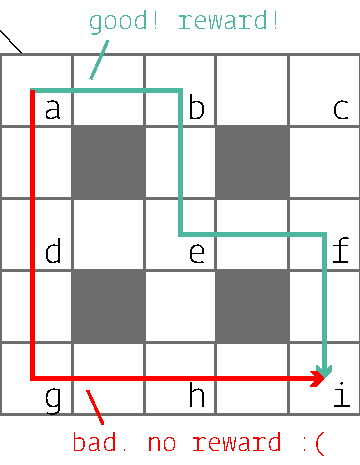
\includegraphics[]{figures/side_18_maze.pdf}
\caption{The subject must reach point \texttt{i} but only via the correct (green) path.}
\label{fig:maze}
\end{marginfigure}

In Autopilot, we would define a hardware object that logs positions from the actimeter with a \mintinline{python}{store_position()} method. If the animal has entered the target position ("i" in this example), a \mintinline{python}{task_trigger()} that advances the task stage is called. The following code is incomplete, but illustrates the principle.

\begin{pythoncode*}{label= \texttt{\textbf{maze - hardware}}}
class Actimeter(Hardware):
    def __init__(self):
        # ... some code to access the hardware ...
        self.positions = []
        self.target_position = "i"
        
    def store_position(self, position):
        self.positions.append(position)
        
        if position == self.target_position:
            self.finished_cb(self.positions) |$\tikzmark{finishcb}$|
            self.positions = []
\end{pythoncode*}
%
\begin{tikzpicture}[overlay, remember picture]
\draw[<-] (pic cs:finishcb) ++(0,0.1) to[left] ++(3.1,0)node[below right, yshift=8pt, text width=2.4in]{See line \ref{callback} below};
\end{tikzpicture}

\vspace{-12pt}

The task follows, with parameters and network methods for sending data omitted for clarity.

\begin{pythoncode*}{label= \texttt{\textbf{maze - task}}, firstnumber=last}
class Maze(Task):
    def __init__(self):
        self.target_path = ['a', 'b', 'e', 'f', 'i']
        
        self.actimeter = Actimeter()
        self.actimeter.finished_cb = self.finished |$\tikzmark{callback}\label{callback}$|
        
    def finished(self, positions):
        if positions == self.target_path: |$\tikzmark{equality}$|
            self.reward()
\end{pythoncode*}

\begin{tikzpicture}[overlay, remember picture]
\draw[<-] (pic cs:callback) ++(0,0.1) to[left] ++(1.8,0) --++(0,1.5) --++(0.2,0)node[below right, yshift=8pt, text width=2.4in]{The actimeter is given a reference to the Maze task's \mintinline{python}{finished()} method, which it calls when the target position is reached};
\draw[<-] (pic cs:equality) ++(0,0.1) to[left] ++(3.6,0)node[below right, yshift=8pt, text width=2.4in]{The sequence of \texttt{positions} is compared to the \texttt{target\_path} with \texttt{==}. If they match, the subject is rewarded!} ;
\end{tikzpicture}
\vspace{-14pt}

How would such a task be programmed in a finite-state machine formalism? Since the path matters, each "state" needs to consist of the current position and all the positions before it. But, since the animal can double back and have arbitrarily many state transitions before reaching the target corner, this task is impossible to represent with a finite-state machine, as a full representation would necessitate infinitely many states (this is one example of the \textit{pumping lemma}, see \citep{kozenLimitationsFiniteAutomata1997}).

Even if we dramatically simplify the task by 1) assuming the animal never turns back and visits a space twice, and 2) only considering paths that are less than or equal to the length of the correct path, the finite state machine would be as complex as figure \ref{fig:fsmtree}. 

While finite-state machines are relatively easy to implement and work well for simple tasks, they quickly become an impediment to even moderately complex tasks. Even for 2AFC tasks, many desirable features are difficult to implement with a finite state machine, such as: (1) graduation to a more difficult task depending on performance history, (2) adjusting reward volume based on learning rate, (3) selecting or synthesizing upcoming stimuli based on patterns of errors\citep{bakAdaptiveOptimalTraining2016}, etc. 

Some of these problems are avoidable by using extended versions of finite state machines that allow for extra-state logic, but require additional complexity in the code running the state machines to accomodate, and with enough exceptions the clean systematicity that is the primary benefit of finite state machines is lost. Autopilot attempts to avoid these problems by providing \textit{tools} to program tasks without \textit{requiring a specified format}, balancing the increased complexity by scaffolding the broader ecosystem of the experiment like its output data, hardware control, etc. When possible, we have tried to avoid forcing people to change the way they think about their work to fit our "little universe"\sidenote[][-6.5cm]{We take inspiration from Aaron Swartz' description of another engineering project, the Semantic Web, that became too precious about its formalisms:\\"Instead of the “let’s just build something that works” attitude that made the Web (and the Internet) such a roaring success [...] they formed committees to form working groups to write drafts of ontologies that carefully listed (in 100-page Word documents) all possible things in the universe and the various properties they could have, and they spent hours in Talmudic debates over whether a washing machine was a kitchen appliance or a household cleaning device. [...] And instead of spending time building things, they’ve convinced people interested in these ideas that the first thing we need to do is write \textit{standards.} (To engineers, this is absurd from the start—standards are things you write \textit{after} you’ve got something working, not before!)"\citep{swartzAaronSwartzProgrammable2013}} and instead try to provide a set of tools that let researchers decide how they want to use them.

\begin{figure*}[hb!]
\caption{State transition tree for a simplified maze task.}
\label{fig:fsmtree}
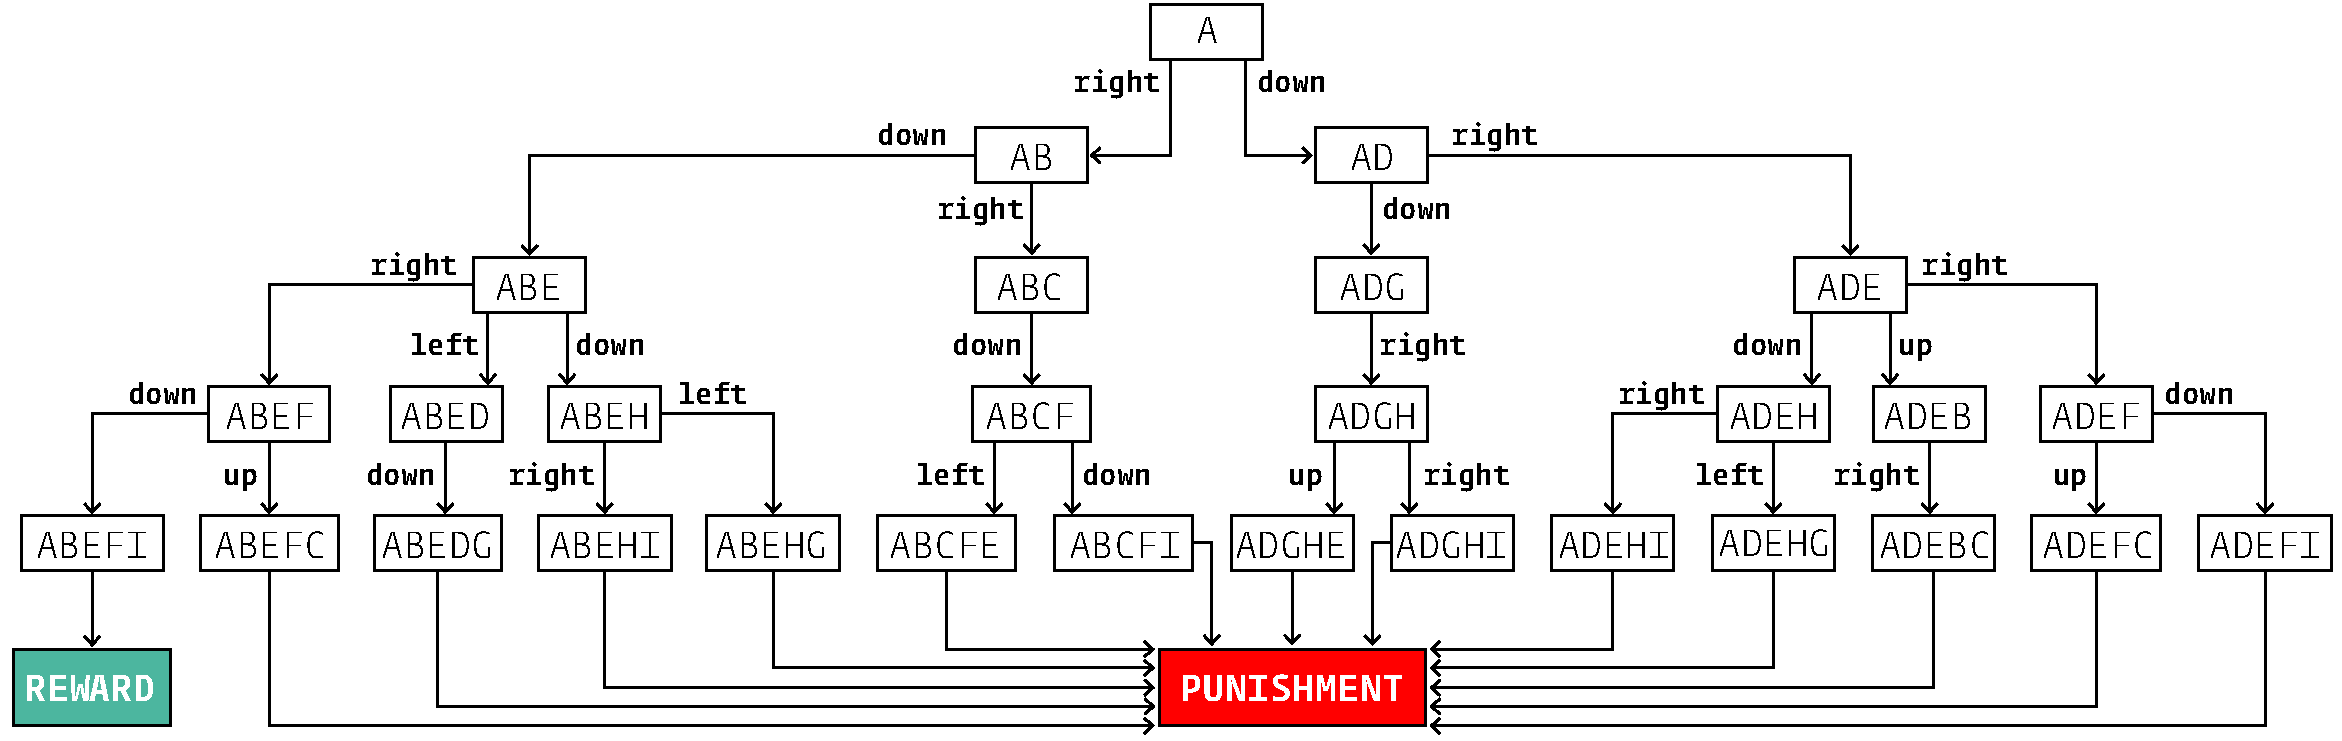
\includegraphics[]{figures/maze.pdf}
\end{figure*}


\clearpage
